\section{General purpose GPU computing}

As the dimensionality of a problem increases, so often too does the time required for performing simulations. It can become necessary to find ways of optimising the use of computational resources to reach a final result in a much shorter amount of time. One such method for accelerating numerical solutions involves the use of multiple compute cores on a central processing unit (CPU) operating independently on different data elements in unison. This form of parallel computation can be achieved through the use of the OpenMP (Open Multi-Processing) application programming interface (API), which defines how a program may parallelise certain elements of code. It allows the developer to fully utilise the power of a multicore processor. However, the limit on how much performance can be gained by this method is set by the number of compute cores available to the system. It should also be noted that MATLAB has inherent support for such programming paradigms, and fully abstracts the implementation from the developer. Therefore, in this instance using such a means of parallelisation would not be very beneficial <!!!why not?!!!>.

Another widely used programming paradigm is that of MPI (message passing interface). Where OpenMP allows a user to utilise all available processors on a single system, MPI allows the use of an (almost) unlimited number of computer systems operating in parallel together, each known as a node. This is the method generally preferred in programs written for compute clusters, where a large number of nodes are available to use. It is preferable for applications that have minimal dependence between data, as a compute bottleneck may occur if data spread over multiple nodes is required for an operation. This would require continual transmission of data between individual nodes, which (at current data rates) would be limited to bus speeds of (assuming Infiniband optical connections) on the order of ten gigabytes per second. Compared to a local calculation requiring little to no transfers, the memory bandwidth can be (assuming current high performance 12 core processors) as high as 60 gigabytes per second \cite{DAT:Intel_xeon}. Therefore, it is important to note that transfers should be minimised to avoid bottlenecks, but transfers are often necessary to make use of the large number of processing cores required to obtain results within short timescales. Therefore, to give a significant performance benefit, a large number of cores, a high memory bandwidth, a high-speed interconnect between cores (nodes), as well as sufficient space to store the problem in memory are required.

One possible means of achieving this high performance is through the use of graphics processing units (GPUs). GPUs are signal processing devices, and have been highly developed over the past 20 years to offload much of the computation required to display images from the central processing unit (CPU). As a result, GPUs have been given the task of performing operations necessary to update a large number of pixels in a short amount of time, as well complex 3D math for image rendering. This has been achieved through giving the GPUs a large number of specialised compute cores for floating-point arithmetic, effectively operating in parallel. With the advent of general purpose GPU (GPGPU) computing, the ability to exploit these cores for the purpose of numerical computing has become possible. A problem can be mapped to the hardware of a GPU, and all parallelisable operations can be accelerated, reducing the overall compute overhead required for evaluating results. For the latest generation of industry standard GPUs used in computational acceleration the memory bandwidth for the device global memory (equivalent of RAM) is given as 288 gigabytes per second, with almost 3000 cores on demand, yielding a theoretical total of $1.41\times10^{12}$, floating-point operations per second (FLOPS), following the formula
\begin{equation}
    \text{FLOPS} = \text{cores}\times\text{clock freq.}\times\text{ops. per clock cycle}.
\end{equation}

In comparison to this are Intel Xeon CPU throughput values, which yield approximately $1\times10^{11}$ FLOPS. As can be seen, performance of an order of magnitude can be gained by using a GPU for calculations, over high-performance (Xeon) CPUs. This has been shown to allow for effective implementation of the previously mentioned Fourier split-operator method \cite{Num:Bauke_cpc_2011}, and we have shown that it yields performance exceeding that of CPU's for a modest choice of GPU \cite{AO:Morgan_ORiordan_pra_2013}.


\subsection{Parallel operations}
\label{sub:Parallel operations}
For a calculation to fully utilise all available throughput of a parallel-capable
compute device, it is essential to break down the problem into easily parallelised (emabarrassingly parallel) sub-problems. Considering summation as an example, imagine we have a large vector of floating point values that are to be summed together. The traditional way to solve this would be to iteratively add values to an accumulator, and return the final value at the end as the sum. This simple algorithm is $\mathcal{O}(n)$ complexity, as we iterate through each element at a time. Given that summation is associative, we easily parallelise this operation. By dividing our vector amongst a number of available processing cores recursively, we can reduce the computation to $\mathcal{O}(\log{} n)$. This algorithm can give a significant benefit when a large number of summations are performed.

Another typical algorithm following this logic is the Hadamard product (element-wise multiplication) of two vectors, or matices. Although in parallel the number of operations and complexity remains the same, the advantage comes from the lack of interdependence between elements. The multiplications can be carried out asynchronously, allowing all freely available cores to work continuously until every element pair is multiplied.

\begin{figure}
    \centering
    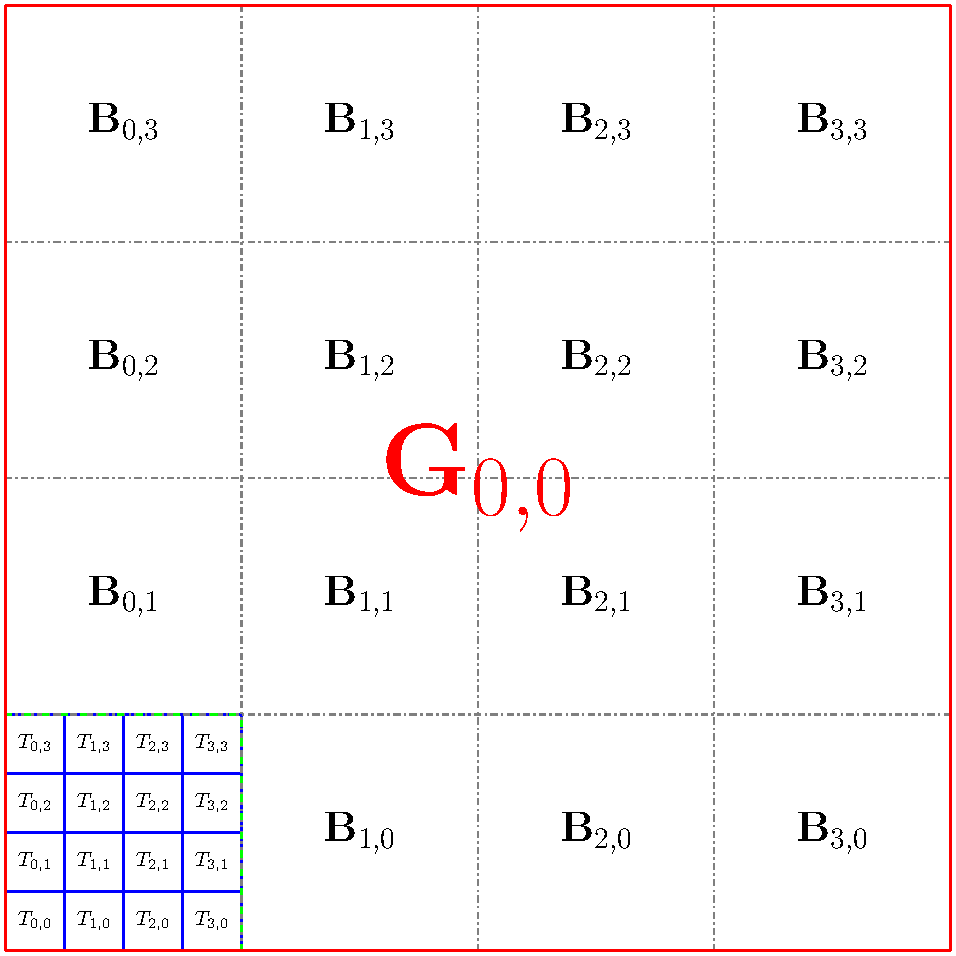
\includegraphics[scale=0.5]{./ch2_numerics/CUDA/gputhreads.pdf}
    \caption{GPU threads, blocks, grid breakdown.}
    \label{fig:gpu_threads}
\end{figure}

Given that GPUs are first and foremost image processing devices, their ability to perform Fourier transforms rapidly should be a well developed strength. It is. Given the large number of available cores, FFTs can be significantly faster on a GPU than performing the same operation on many CPUs \cite{AO:Morgan_ORiordan_pra_2013}. The CUFFT (Cuda FFT) library allows for a seamless way to take advantage of this performance increase using GPUs, with performance gains discussed in the following section.

\section{3D STIRAP using GPU}
For performance metrics, I will discuss the use of a GPU-enabled Schrodinger equation integrator developed by myself, comparing the results to a multi-core MPI enabled version by T. Morgan and N. Crowley. We solved the Schrodinger equation for a fully three-dimensional potential, demonstrating its accuracy and improved performance compared to standard HPC methods.
